\cia\vspace{-2 cm}
\section{Acceptance calculation}
In each bin considered for the analysis (see Section \ref{sec:binning})
the acceptance $A$ is the ration of the number $R$ of generated events 
to the number $G$ of generated events:
\begin{equation}
A=\Dfrac{R}{G}
\end{equation}



\begin{figure}[h]
 \begin{center}
  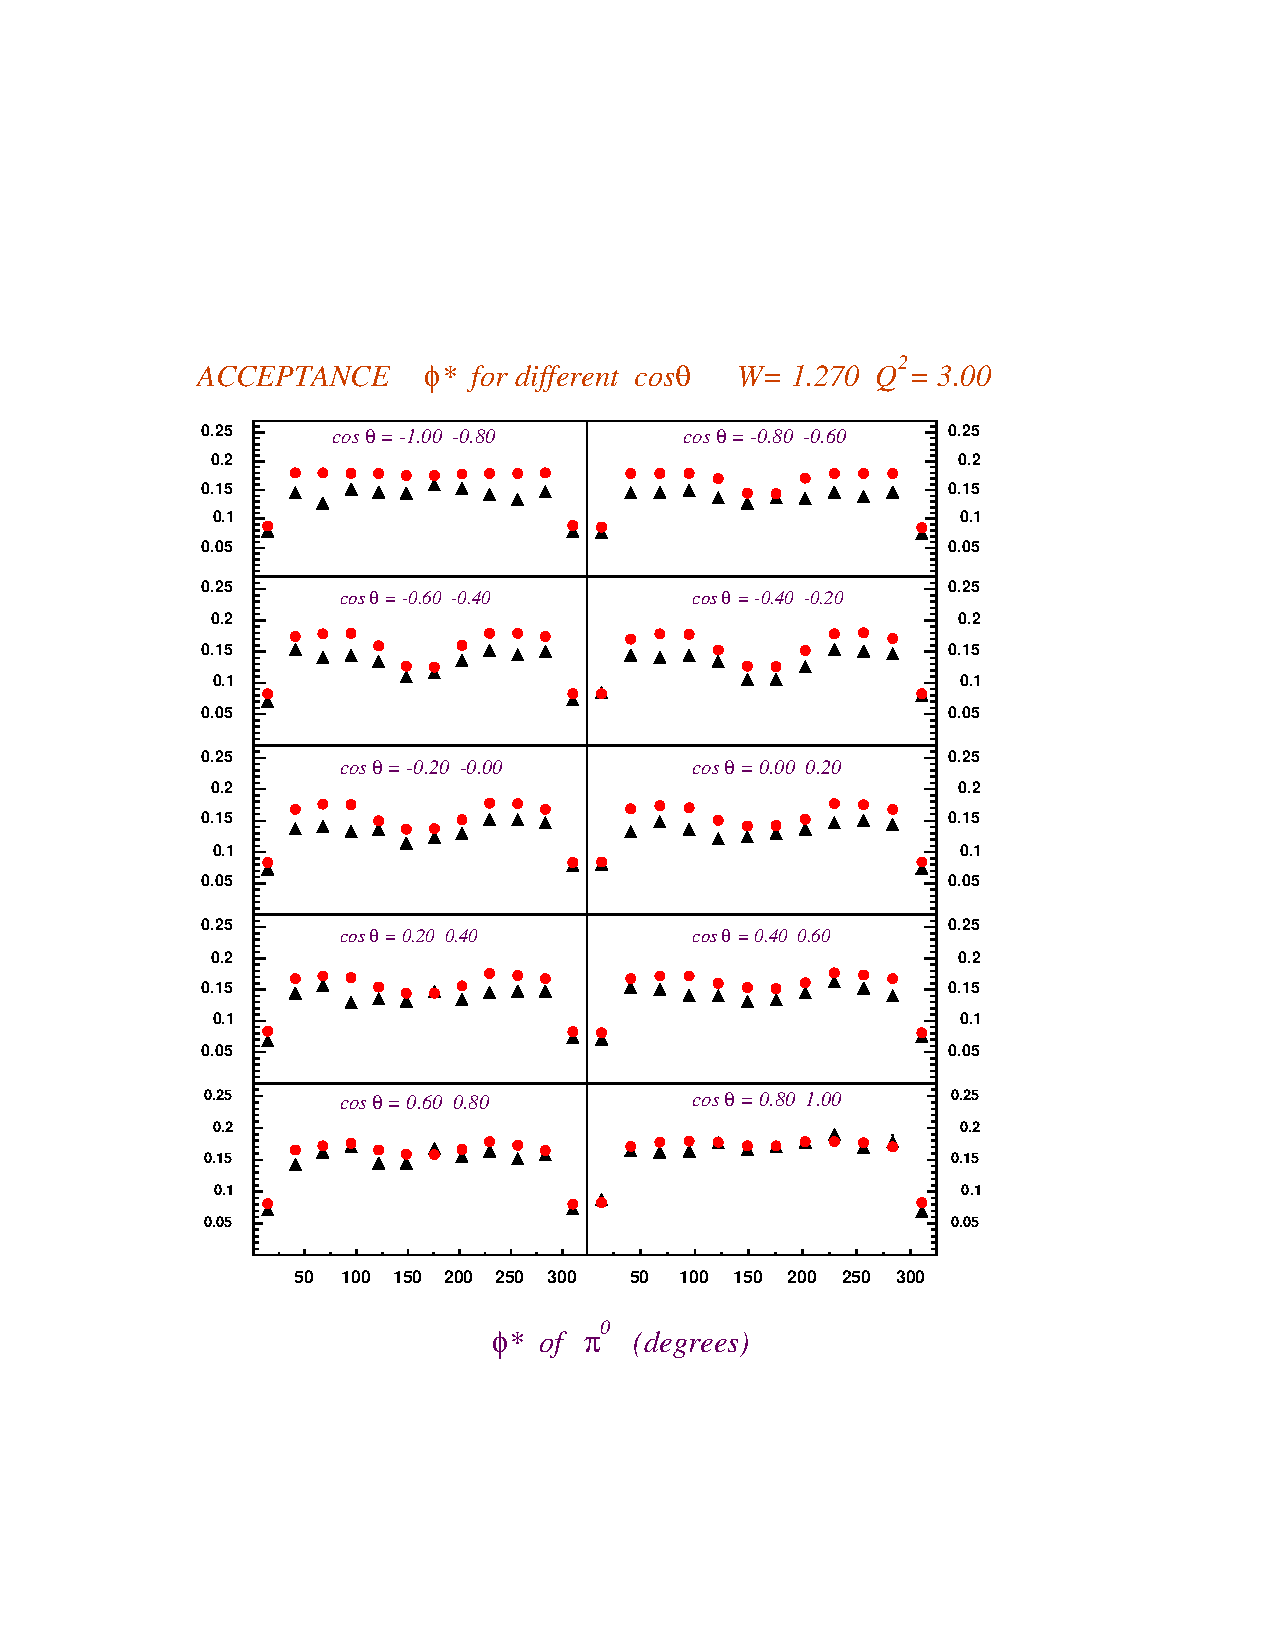
\includegraphics[width=15cm, bb=0 120 540 640]{acceptance/img/acc_phi_W1.27_Q23.00}
  \caption[Comparison Geometrical and MonteCarlo acceptances, $1.26\le W\le 1.28$ GeV and $Q^2=3.0$ GeV$^2$ ]
          { Acceptance calculation for $1.26\le W\le 1.28$ GeV and $Q^2=3.0$ GeV$^2$. Red: geometrical 
	             acceptance. Black: MonteCarlo acceptance.}
 \label{fig:accept1}
  \end{center} 
\end{figure} 

In \F{fig:accept1} and \F{fig:accept2} the acceptance (black triangles)
is shown as a function of $\phi^*$ for different $\cos\theta^*$. 
The geometrical acceptance (red points)
is shown for comparison.

The difference between the two distributions is due to various effects
as detector efficiency, bin migration, detector resolution.




\begin{figure}[h]
 \begin{center}
  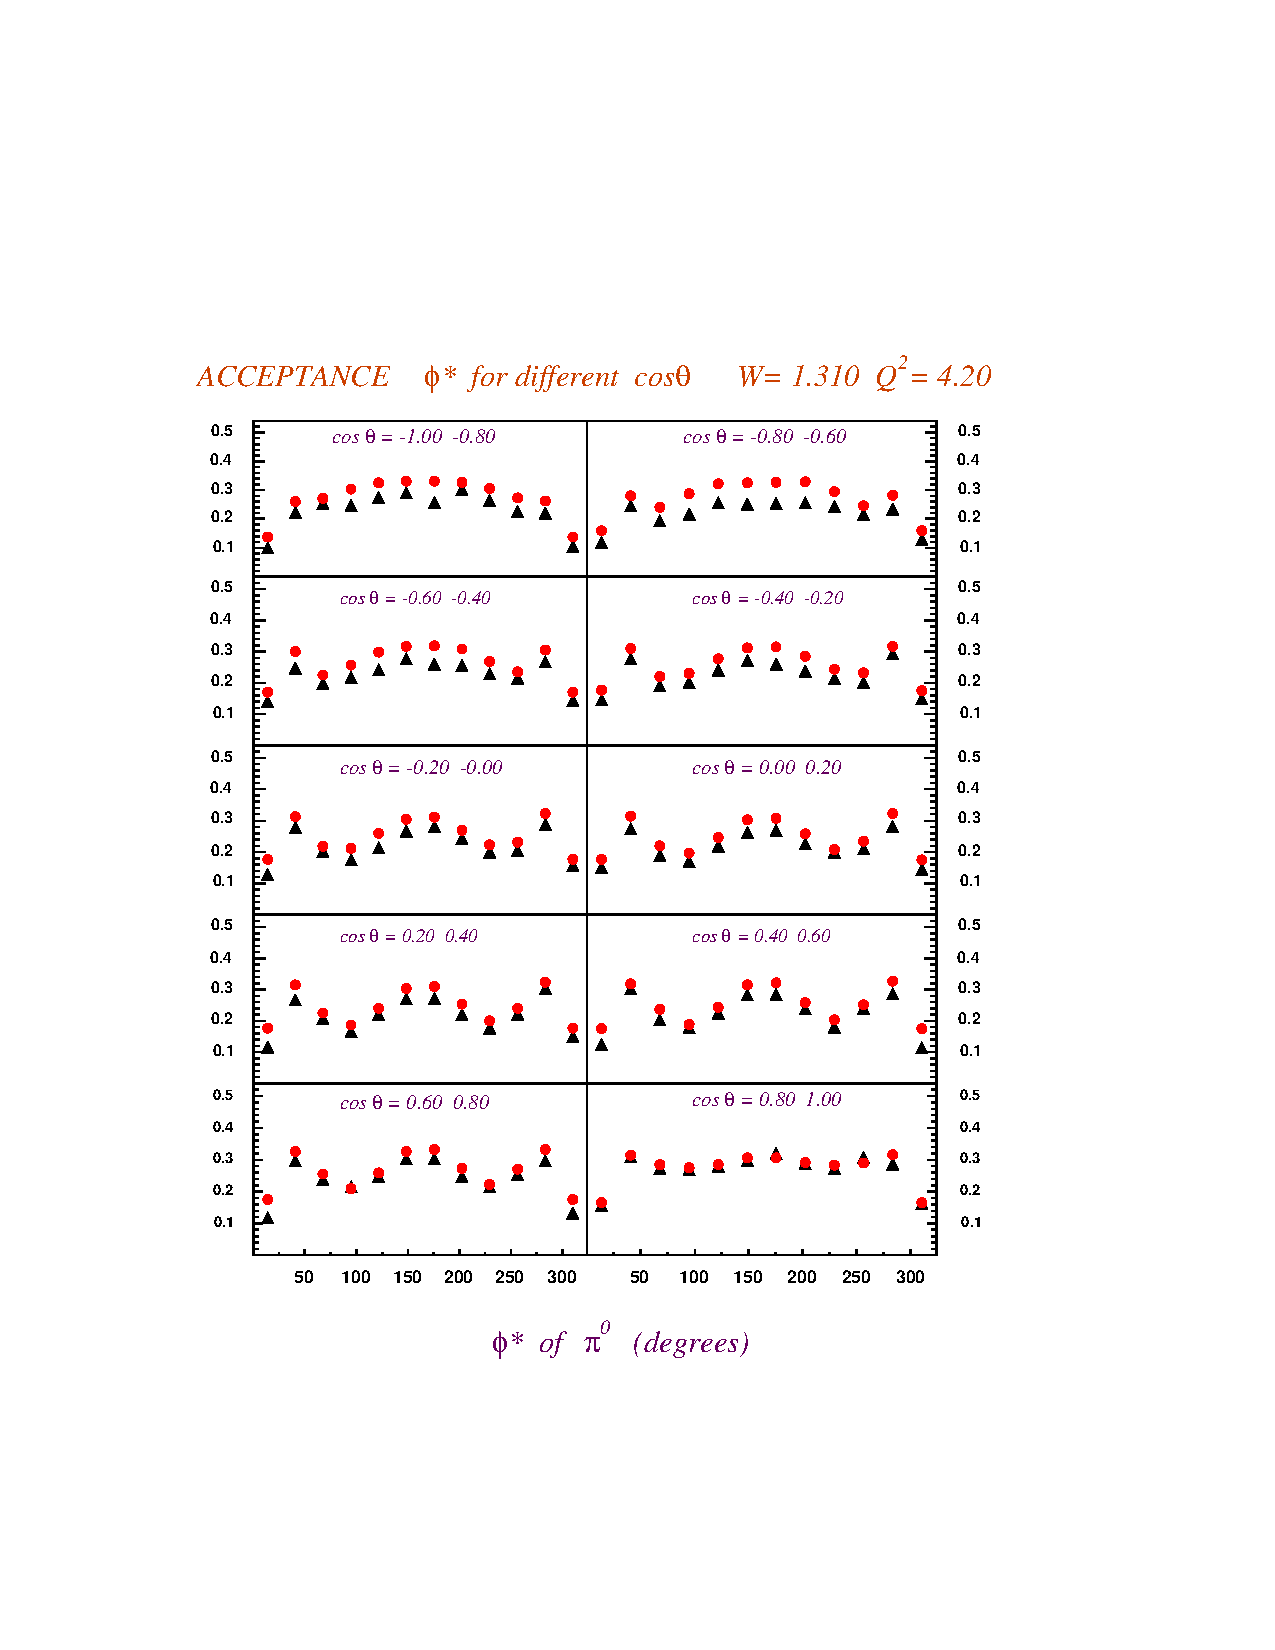
\includegraphics[width=15cm, bb=0 120 540 640]{acceptance/img/acc_phi_W1.31_Q24.20}
  \caption[Comparison Geometrical and MonteCarlo acceptances, $1.30\le W\le 1.32$ GeV and $Q^2=4.2$ GeV$^2$]
          { Acceptance calculation for $1.30\le W\le 1.32$ GeV and $Q^2=4.2$ GeV$^2$. Red: geometrical 
	             acceptance. Black: MonteCarlo acceptance.}
 \label{fig:accept2}
  \end{center} 
\end{figure} 

See    \begin{verbatim} 
http://www.jlab.org/~ungaro/pi0eprod/acc_plots
\end{verbatim}
for the acceptance correction in each bin considered as a function of $\phi^*$ or $\cos\theta^*$.














